\section{What an off line zero would do}\label{ch:offline}



The distances of Section~\ref{ch:distances} compare $\mu_\varepsilon$ with $U_{\RH}$ on a window where the zeros are known to lie on the line, and there the matched distance leaves only a numerical floor. How each distance would change if a zero left the line can be computed in closed form, because by Proposition~\ref{prop:struct} an off line zero at distance $\delta$ from the line enters the Thorin density, together with its reflection in the line, only through the kernels $P_{\varepsilon+\delta}+P_{\varepsilon-\delta}$ at its ordinate, the second of which is negative once $\varepsilon<\delta$. Proposition~\ref{prop:signature} computes the effect for a displacement that keeps the count, for a pair missing from a list of line zeros, and for the negative mass of a displaced zero. Together the three signatures show that an off line zero is most visible at resolutions comparable to its distance from the line, a theme that returns in Section~\ref{ch:finite}. Read against the floor of the matched distance, they give detection thresholds below height $200$ and a calibration of the method above it.

\subsection{Three signatures of an off line zero}\label{sec:ch8:signatures}

Off line zeros come in pairs $\tfrac12\pm\delta+i\gamma$ with $0<\delta<\tfrac12$, together with their conjugates, and near $\gamma$ a pair contributes $P_{\varepsilon+\delta}+P_{\varepsilon-\delta}$ to $\rho_\varepsilon$ where two line zeros would contribute $2P_\varepsilon$. A displacement that keeps the count $N(T)$ therefore moves two line zeros at height $\gamma$ to such a pair, as a double zero does at a collision in the de Bruijn Newman flow (Section~\ref{ch:dbn}). Parts (i) and (iii) of Proposition~\ref{prop:signature} are normalised per displaced zero, and part (ii) per pair.

\begin{proposition}\label{prop:signature}
Let $\varepsilon>0$ and $0<\delta<\tfrac12$; when $\delta=\varepsilon$, $P_0$ denotes the unit point mass at the origin.
\begin{enumerate}
\item[(i)] (Displaced zeros, same count.) If two line zeros at height $\gamma$ are replaced by the quadruple $\tfrac12\pm\delta\pm i\gamma$, the density near $\gamma$ changes by $2g$, where $g=\tfrac12(P_{\varepsilon+\delta}+P_{\varepsilon-\delta})-P_\varepsilon$ is the change per displaced zero, and
\[
\tv{g}=\frac{3\sqrt3}{4\pi}\Big(\frac\delta\varepsilon\Big)^2+O\Big(\frac{\delta^4}{\varepsilon^4}\Big),\qquad \delta<\varepsilon .
\]
\item[(ii)] (Pair omitted from the list.) If a pair at $\tfrac12\pm\delta+i\gamma$ exists but a list of line zeros omits it, the difference is $P_{\varepsilon+\delta}+P_{\varepsilon-\delta}$ and
\[
\tv{P_{\varepsilon+\delta}+P_{\varepsilon-\delta}}=\begin{cases}2,&\delta\le\varepsilon,\\[2pt] \dfrac8\pi\arctan\sqrt{\dfrac{\delta+\varepsilon}{\delta-\varepsilon}}-2,&\delta>\varepsilon.\end{cases}
\]
\item[(iii)] (Negative mass.) For $\delta>\varepsilon$ the negative part of $\tfrac12(P_{\varepsilon+\delta}+P_{\varepsilon-\delta})$, the density of one displaced zero, has mass \[\frac2\pi\arctan\sqrt{\frac{\delta+\varepsilon}{\delta-\varepsilon}}-\frac12=\frac{\varepsilon}{\pi\delta}+O\Big(\frac{\varepsilon^3}{\delta^3}\Big).\]
\end{enumerate}
\end{proposition}

\begin{proof}
(i) Taylor expansion in $\delta$ gives $g=\tfrac{\delta^2}{2}\partial_a^2P_a|_{a=\varepsilon}+O(\delta^4)$ \cite[Proposition 19.7]{P26}, with a remainder of $L^1$ norm $O(\delta^4/\varepsilon^4)$. Since $\partial_a^2P_a(x)=(2a/\pi)(a^2-3x^2)/(a^2+x^2)^3$, the substitution $x=\varepsilon v$ gives $\partial_a^2P_a|_{a=\varepsilon}=2(1-3v^2)/(\pi\varepsilon^3(1+v^2)^3)$ and $dx=\varepsilon\,dv$. The function $(1-3v^2)/(1+v^2)^3$ is the derivative of $v/(1+v^2)^2$, whose total variation is four times its maximum $9/(16\sqrt3)$, that is $3\sqrt3/4$, so the $L^1$ norm of $\partial_a^2P_a$ at $a=\varepsilon$ is $(2/(\pi\varepsilon^2))\cdot3\sqrt3/4=\frac{3\sqrt3}{2\pi\varepsilon^2}$, and multiplying by $\delta^2/2$ gives (i).
(ii) For $\delta\le\varepsilon$ both kernels are nonnegative with mass one. For $\delta>\varepsilon$ put $a=\delta+\varepsilon$, $b=\delta-\varepsilon$, so the difference is $P_a-P_b$, which is negative exactly on $|x|<\sqrt{ab}$. Integrating, $\tv{P_a-P_b}=\frac4\pi[\arctan\sqrt{a/b}-\arctan\sqrt{b/a}]$, and $\arctan y+\arctan(1/y)=\pi/2$.
(iii) $P_a-P_b$ has total mass zero, so its negative part is half its norm; halve again for the factor $\tfrac12$.
\end{proof}

With $\varepsilon/\delta=\sin\phi$ one has $\arctan\sqrt{(\delta+\varepsilon)/(\delta-\varepsilon)}=\pi/4+\phi/2$, so for $\delta>\varepsilon$ the norm in (ii) is $(4/\pi)\arcsin(\varepsilon/\delta)$ and the mass in (iii) is $(1/\pi)\arcsin(\varepsilon/\delta)$. In part (i) the list is correct in number but two of its zeros have left the line, and the density differs from the Poisson smoothing of the list by $2g$, which to leading order is $\delta^2\partial_a^2P_a$ at $a=\varepsilon$, quadratic in the displacement. In part (ii) the list omits the pair; the difference is of order one while the resolution is coarser than the displacement, and fades like $4\varepsilon/(\pi\delta)$ once it is finer. Part (iii) bounds the negative mass that a displaced zero can contribute, which also fades like $\varepsilon/\delta$. Figure~\ref{fig:sensitivity} plots the three signatures.

\begin{figure}[t]
\centering
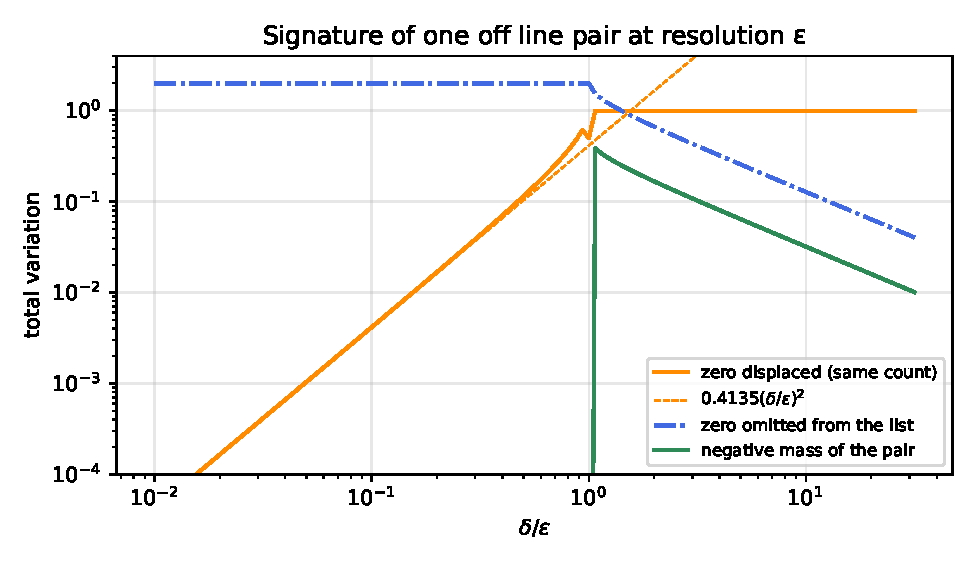
\includegraphics[width=0.7\textwidth]{fig/sensitivity.pdf}
\caption{The three signatures of Proposition~\ref{prop:signature} as functions of $\delta/\varepsilon$: $\tv{g}$ per displaced zero (part (i)), with its leading term $0.4135(\delta/\varepsilon)^2=(3\sqrt3/(4\pi))(\delta/\varepsilon)^2$ dashed; the total variation of an omitted pair (part (ii)); and the negative mass per displaced zero (part (iii)). For $\delta>\varepsilon$, outside the range of part (i), the kernels of a displaced zero have total mass zero and curve (i) is flat at $1$.}
\label{fig:sensitivity}
\end{figure}

\subsection{Calibration of the matched distance}\label{sec:ch8:calibration}

Proposition~\ref{prop:signature} converts the matched distance of Section~\ref{ch:distances} into detection thresholds. By part (ii), a computed matched distance $\tilde d_{\rm match}(\varepsilon)$ of at most $3.7\times10^{-9}\,\varepsilon$ excludes any omitted pair with ordinate in $(0,200)$: such a pair contributes total variation $(4/\pi)\arcsin(\varepsilon/\delta)$, or $2$ if $\delta\le\varepsilon$, less only the part of its kernels outside the window. By part (i), a displaced pair that keeps the count adds $2g$ to a difference whose norm is the floor $\tilde d_{\rm match}(\varepsilon)$, so by the triangle inequality the matched distance rises above the floor as soon as $\tv{g}>\tilde d_{\rm match}(\varepsilon)$, that is, to leading order, once $\delta$ exceeds
\begin{equation}\label{eq:ch8:threshold}
\delta_{\min}(\varepsilon)=\varepsilon\Big(\frac{4\pi\,\tilde d_{\rm match}(\varepsilon)}{3\sqrt3}\Big)^{1/2}.
\end{equation}
With the floors of Table~\ref{tab:tv} this threshold is $3.3\times10^{-5}$ at $\varepsilon=0.5$, $1.1\times10^{-6}$ at $\varepsilon=0.05$ and $3.3\times10^{-8}$ at $\varepsilon=0.005$.

The threshold \eqref{eq:ch8:threshold} is the square root law of \cite[Proposition 19.7]{P26}: the signature grows like the square of the displacement, so the smallest detectable displacement falls like the square root of the achievable distance. The prime side calibration of \cite[Section 19.3.6]{P26} obeys the same law and reaches $\delta\approx0.05$ at $\varepsilon=2$. What changes is the reach: the P\'olya route evaluates $\rho_\varepsilon$ at small $\varepsilon$ to about $60$ digits below height $200$ (Section~\ref{sec:ch4:trapezoid}), so the floor is set by the tail model for the zero list (Section~\ref{sec:ch7:matched}) rather than by the evaluator, whereas the prime side is limited by the truncation of Table~\ref{tab:prime}. A positivity test sees less than the matched distance: only the negative part of the whole density, which by part (iii) is at most of order $\varepsilon/\delta$ per displaced zero and which the kernels of the neighbouring zeros can cancel entirely (Section~\ref{ch:finite}). Section~\ref{ch:almost} bounds the mass of the negative part of the density below a given height by the number of zeros to the right of the basepoint and, through zero density estimates, shows with no hypothesis that it is a vanishing fraction of the positive part.

These thresholds concern zeros below height $200$, where the argument principle count is already decisive, and their use is to calibrate the method above the verified window. There the cost per point of the P\'olya route grows with the height (Section~\ref{sec:ch6:measure}), and the count itself must come from the argument of $\xi$, which Section~\ref{ch:turing} reads from the Thorin mass (Proposition~\ref{prop:zerodensity}).
